\subsection{GPU Force Calculation Kernel}

In the original GPU kernel implementation, each thread block calculates the forces on the atoms in one patch (patch 1)
due to the atoms in another patch (patch 2). Fig.~\ref{figs:pseudocode} presents the pseudo-code for kernel calculation.
In the outer loop, each thread copies atoms from patch 1 to local registers. In the inner loop. threads in the block collaborate to
load atoms from patch 2 to shared memory. Before and after reading of atoms in patch 2, there are synchronization calls to guarantee
that data is ready to be used before the calculation and is ready to be rewritten after the calculation. During the force
calculation phase, each thread iterates atoms in patch 2 and computes the distance with current atom in patch 1.
If the distance is within cut-off distance, it accumulates the forces for the current atom in patch 1 and finally writes force results
back to GPU global memory. The kernel also calculate a pairlist every 10 time steps used by following time steps to further avoid redundant work. 

\begin{figure}[h]
\centering
\setlength{\abovecaptionskip}{-1pt}
\setlength{\belowcaptionskip}{-2pt}
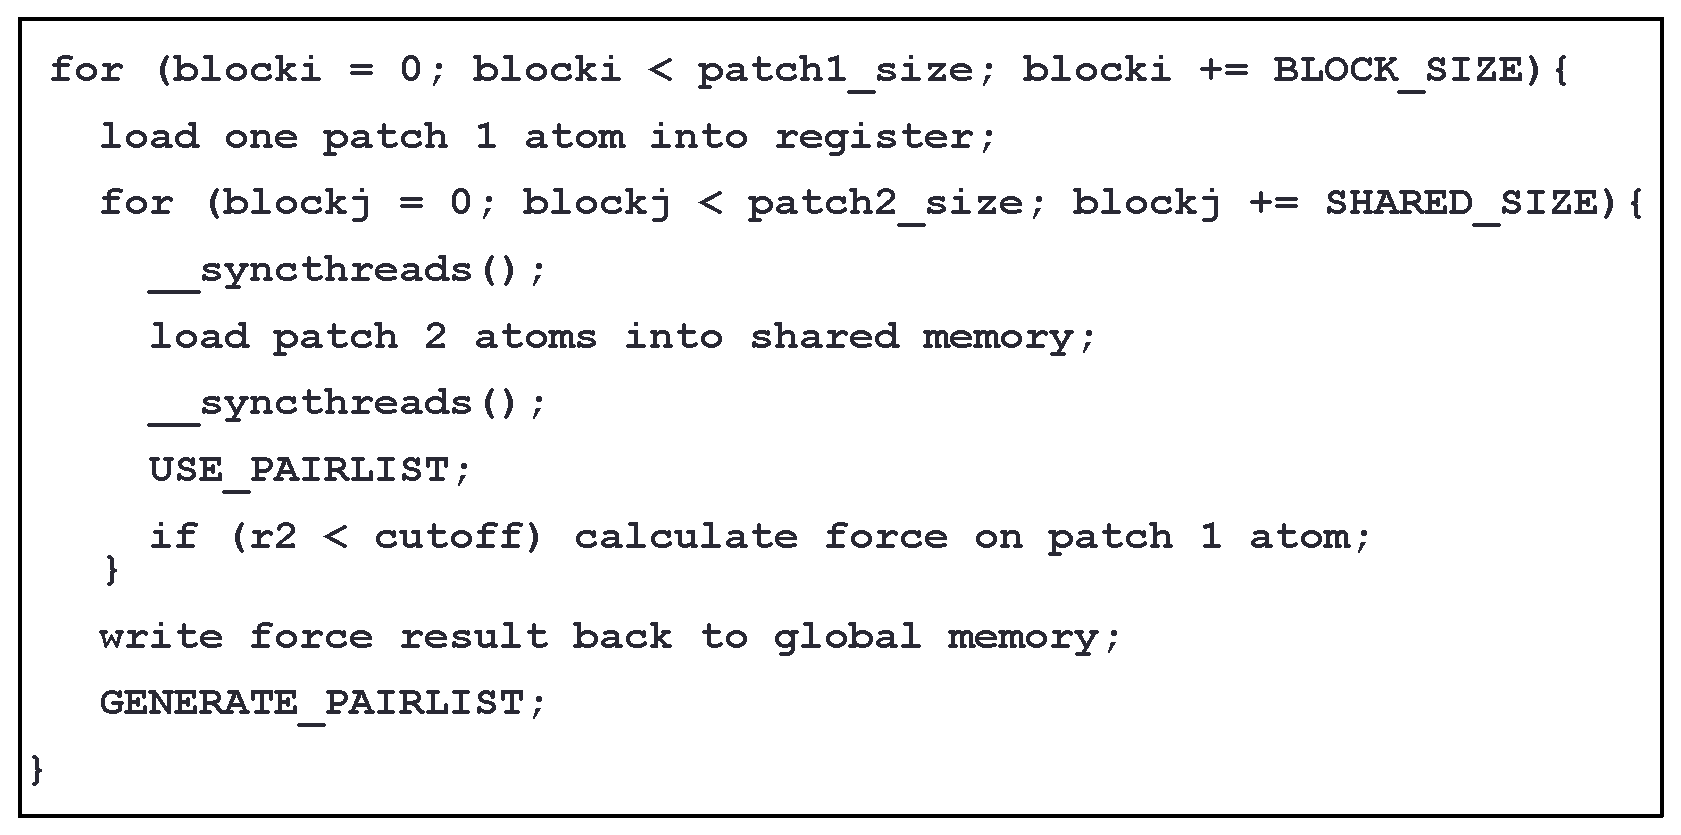
\includegraphics[width=4.0in]{figs/pseudocode.eps}
\caption{Pseudocode for GPU kernel force calculation}
\label{figs:pseudocode}
%\vspace{-0.5cm}
\end{figure}

After profiling the performance of the GPU kernel, we acquired the following observations:
(1) force calculation dominates the most GPU time compared to data loads and stores;
(2) there are great control divergence among different threads due to thread synchronization, which means some threads take a really long time
to reach the synchronization where other threads reach it very quickly. However, all threads in the block have to wait for everyone to
reach the synchronization before they can process further. Besides, use of pairlist may aggravate the divergence.
Based on above observations, we proposed several optimization approaches to reduce the control
divergence. They are described in detail in following sections.

\subsection{Optimizations}
\subsubsection{Patch 1 Atoms Tiling}

As indicated in Fig.~\ref{figs:pseudocode}, in the outer loop, all atoms in patch 2 need to be iterated for each patch 1 atom,
and there will be thread synchonization in every loop. According to that fact, we first considered the optimization of patch 1 atoms tiling,
in which each thread loads mulitple atoms instead of only one from patch 1 in the outer loop. By doing this, total number of outer loops can be reduced.
Because we merge work on each thread, synchronization latency can be decreased as indicated in Fig.~\ref{figs:divergence}.
Furthermore, data reuse can be improved because patch 2 atoms can be used for multiple patch 1 atoms in each outer loop.

\begin{figure}[h]
\centering
\setlength{\abovecaptionskip}{-1pt}
\setlength{\belowcaptionskip}{-2pt}
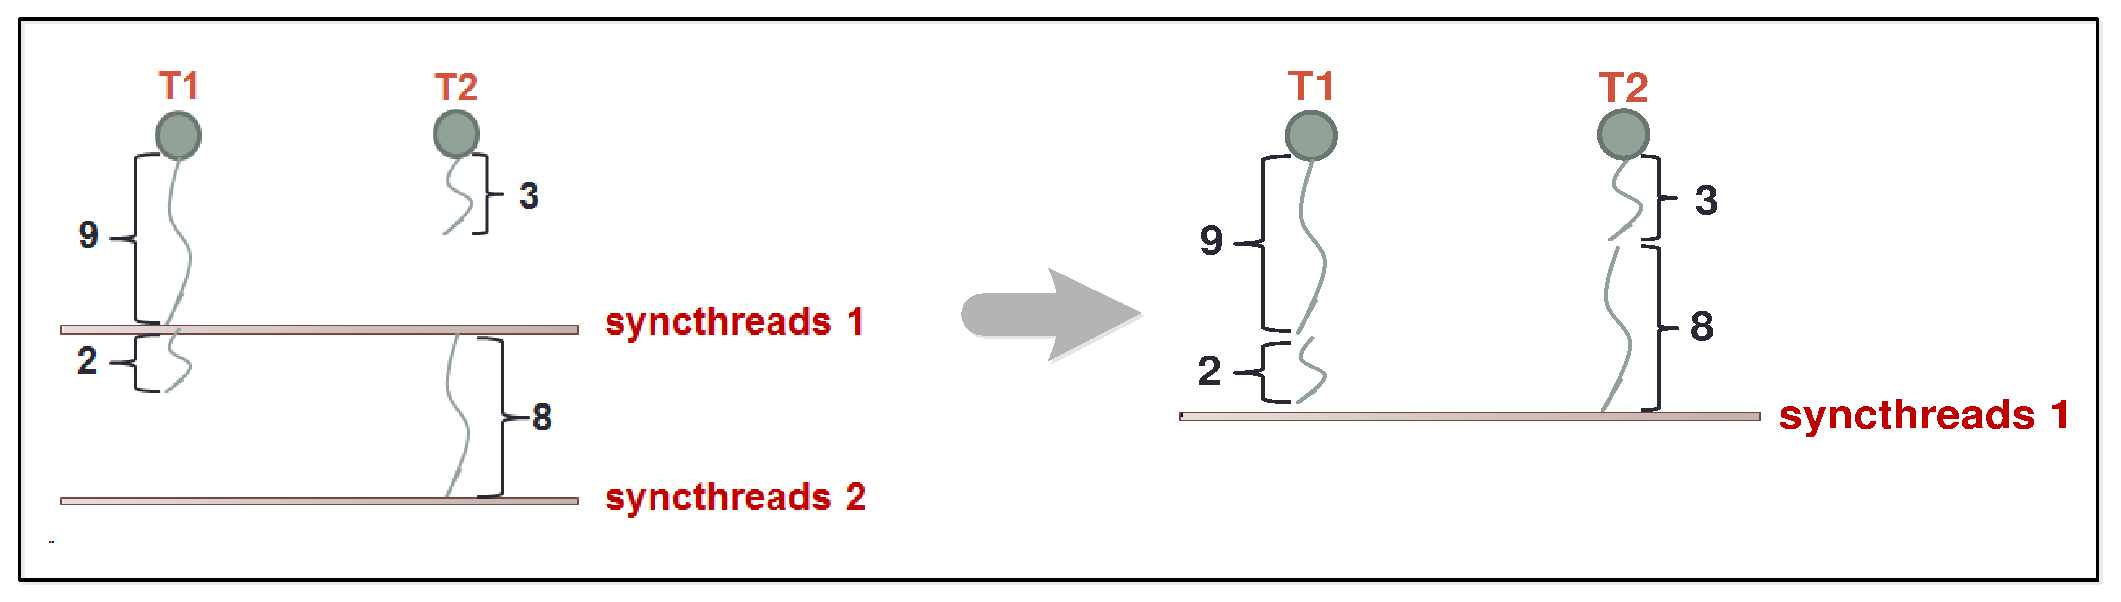
\includegraphics[width=6.0in]{figs/divergence.eps}
\caption{Reduce control divergence by patch 1 tiling}
\label{figs:divergence}
%\vspace{-0.5cm}
\end{figure}

\subsubsection{Patch 2 Atoms Tiling}
We also implemented tiling for loading patch 2 atoms to further reduce synchronization calls. In the original implementation in Fig.~\ref{figs:pseudocode},
for each inner loop, threads collaborate to load patch 2 atoms for one time. Instead, we make threads load multiple times in each inner loop to reduce the
total number of inner loops.

\begin{figure}[h]
\centering
\setlength{\abovecaptionskip}{-1pt}
\setlength{\belowcaptionskip}{-2pt}
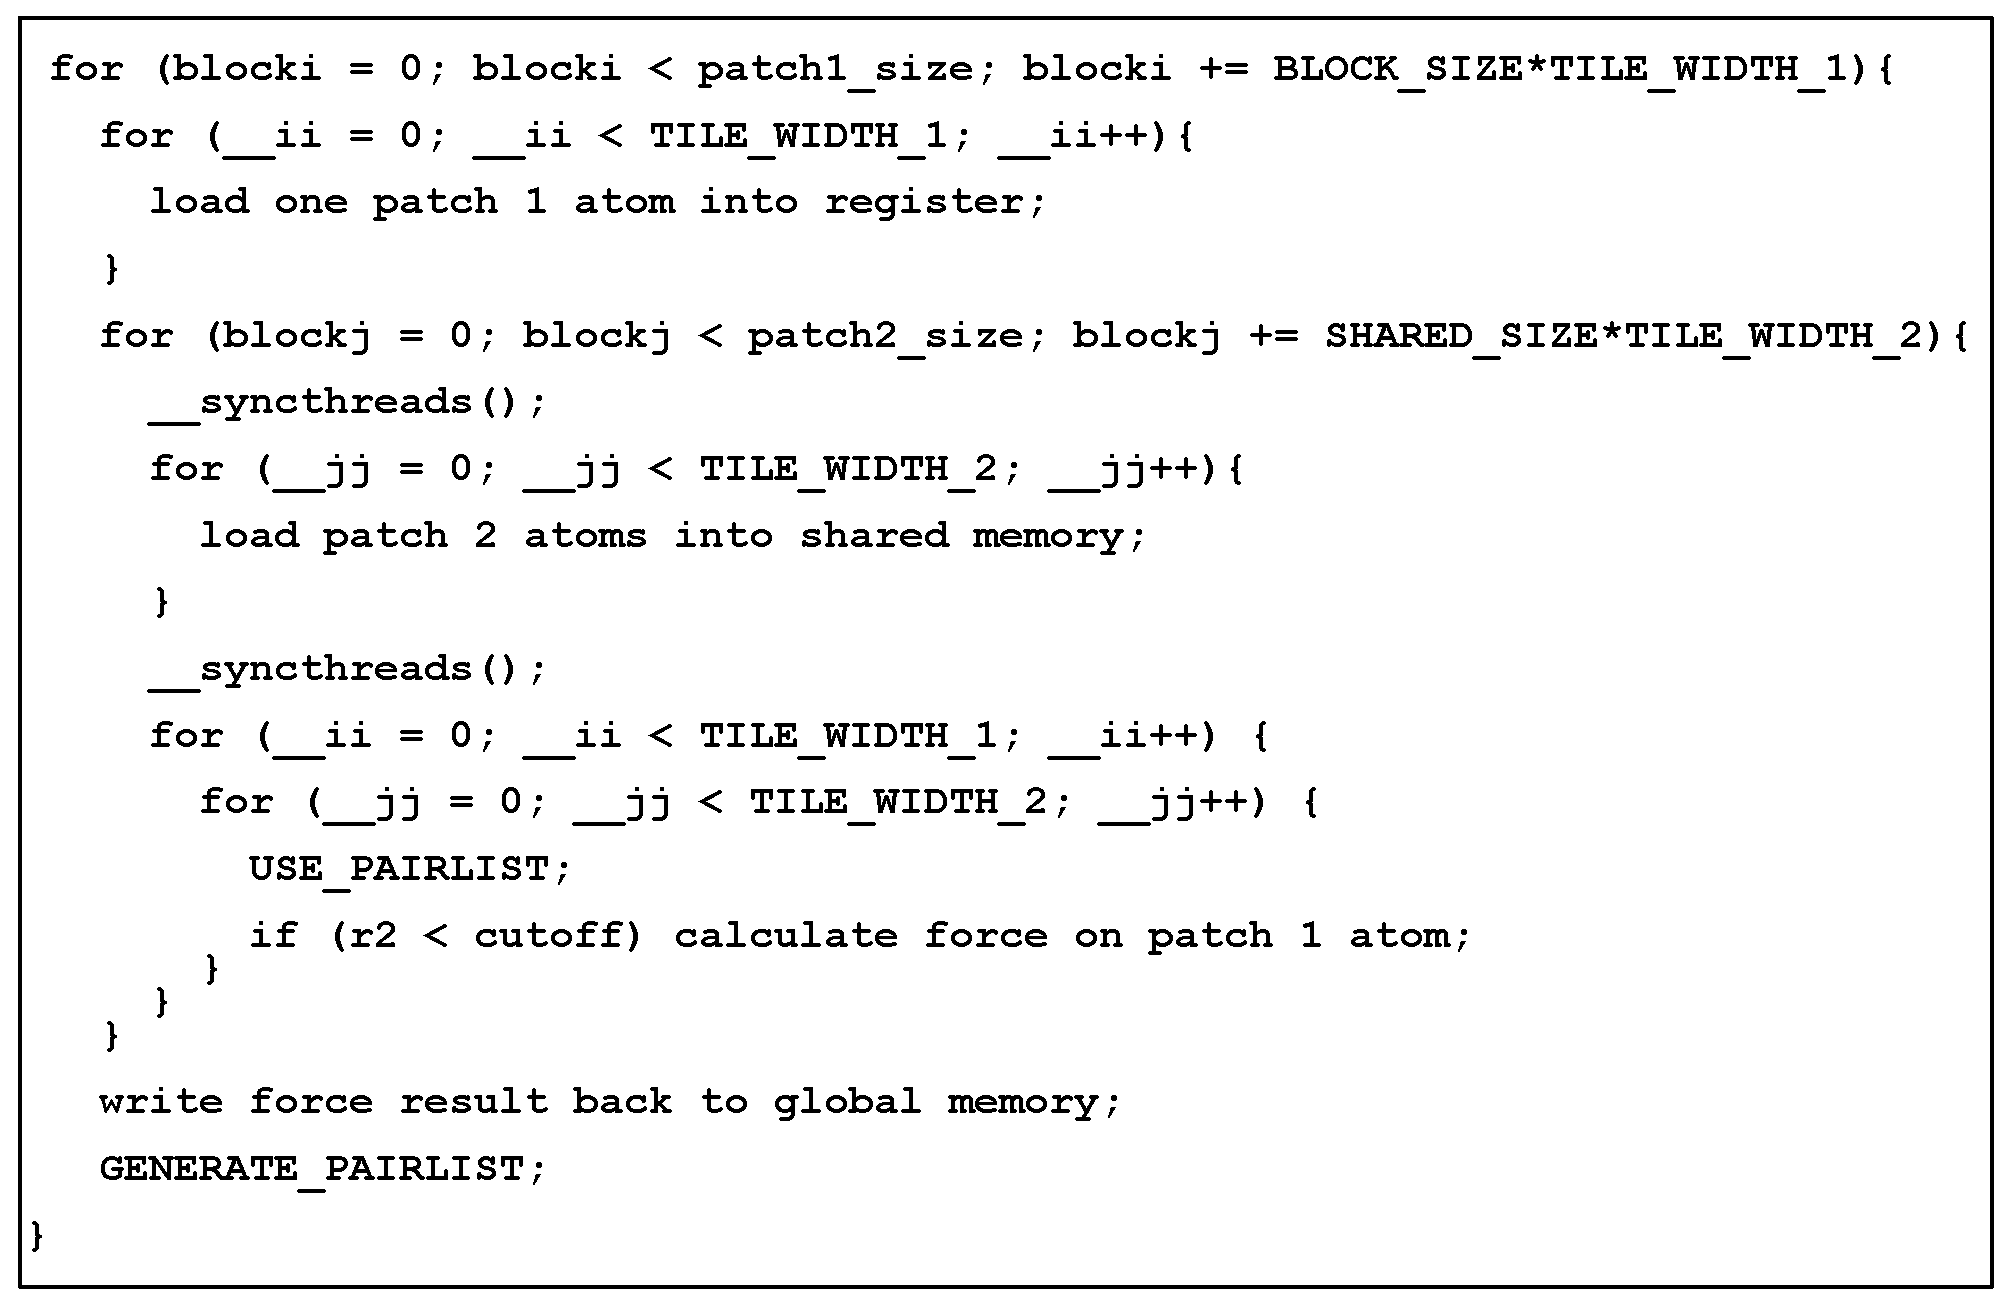
\includegraphics[width=4.0in]{figs/pseudocode-tile.eps}
\caption{Pseudocode for GPU kernel force calculation after tiling optimization}
\label{figs:pseudocode-tile}
%\vspace{-0.5cm}
\end{figure}

\subsubsection{Patch 1 Atoms Sorting}
